%! TeX program = lualatex
\documentclass[a4paper]{article} 

% packages
\usepackage{microtype}      % Slightly tweak font spacing for aesthetics
\usepackage[english]{babel} % Language hyphenation and typographical rules
\usepackage[final, colorlinks = true, urlcolor = black, linkcolor = black]{hyperref} 
\usepackage{changepage}     % adjust margins on the fly

\usepackage{fontspec}
\setmainfont{EB Garamond}
\setmonofont[Scale=MatchLowercase]{Deja Vu Sans Mono}

\usepackage{minted}
\usemintedstyle{algol_nu}
\usepackage{xcolor}

\usepackage{pgfplots}
\pgfplotsset{width=\textwidth,compat=1.9}

\usepackage{caption}
\newenvironment{code}{\captionsetup{type=listing}}{}
\captionsetup[listing]{skip=0pt}
\setlength{\abovecaptionskip}{5pt}
\setlength{\belowcaptionskip}{5pt}

\usepackage[yyyymmdd]{datetime}
\renewcommand{\dateseparator}{--}

\usepackage{titlesec}
% \titleformat{\section}{\LARGE\bfseries}{}{}{}[\titlerule]
% \titleformat{\subsection}{\Large\bfseries}{}{0em}{}
% \titlespacing{\subsection}{0em}{-0.7em}{0em}
%
% \titleformat{\subsubsection}{\large\bfseries}{}{0em}{$\bullet$ }
% \titlespacing{\subsubsection}{1em}{-0.7em}{0em}

% margins
\addtolength{\hoffset}{-2.25cm}
\addtolength{\textwidth}{4.5cm}
\addtolength{\voffset}{-3.25cm}
\addtolength{\textheight}{5cm}
\setlength{\parskip}{0pt}
\setlength{\parindent}{0in}
% \setcounter{secnumdepth}{0}

\begin{document}
\hrule \medskip
\begin{minipage}{0.295\textwidth} 
    \raggedright
    \footnotesize 
    \begin{tabular}{@{}l l}
        Name: & Andrew Hayes \\
        Student ID: & 21321503 \\
        E-mail: & \href{mailto://a.hayes18@universityofgalway.ie}{a.hayes18@universityofgalway.ie} \\
    \end{tabular}
\end{minipage}
\begin{minipage}{0.4\textwidth} 
    \centering 
    \vspace{0.4em}
    \LARGE
    \textsc{ct404} \\ 
\end{minipage}
\begin{minipage}{0.295\textwidth} 
    \raggedleft
    \today
\end{minipage}
\medskip\hrule 
\begin{center}
    \normalsize
    Assignment 2: Image Processing \& Analysis
\end{center}
\hrule

\section{A Morphological Image Processing Pipeline for Medical Images}
\begin{figure}[H]
    \centering
    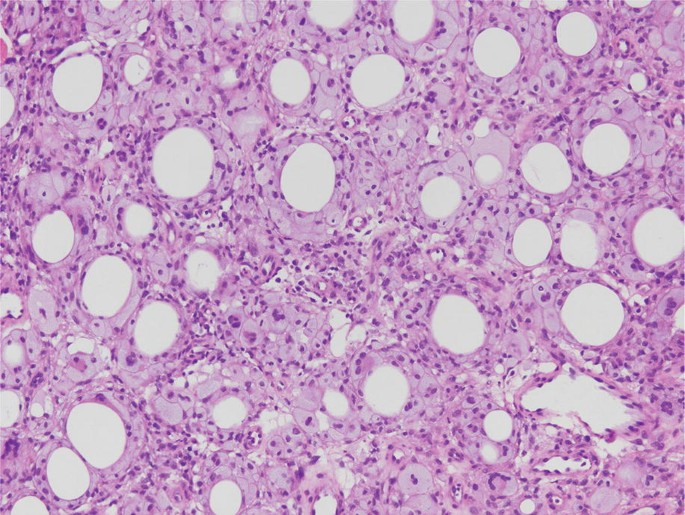
\includegraphics[width=0.7\textwidth]{../Task1.jpg}
    \caption{Original Skin Biopsy Image}
\end{figure}

\subsection{Conversion to A Single-Channel Image}
\begin{code}
\inputminted[linenos, breaklines, frame=single]{python}{../code/task1/1_single_channel_conversion.py}
\caption{\mintinline{python}{1_single_channel_conversion.py}}
\end{code}

Since the image has predominant hues of pink-purple, we would expect the green-channel-only image to be the one that yields the highest contrast, as pink \& purple colours are made up primarily by the blue \& red channels: the dominance of these channels results in little variance in intensity within these channels, and therefore green will have the highest intensity variance.
This is proven true by the text output of the above code, where the standard deviation of the greyscale image based off the green channel alone is by far the highest:
\begin{figure}[H]
    \centering
    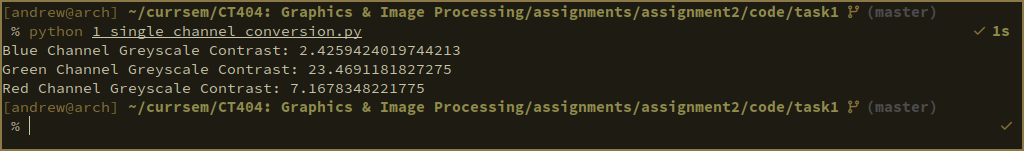
\includegraphics[width=\textwidth]{./images/1_single_channel_conversion_output.png}
    \caption{Output of \mintinline{python}{1_single_channel_conversion.py}}
\end{figure}

\noindent
\begin{minipage}{0.24\textwidth}
    \centering
    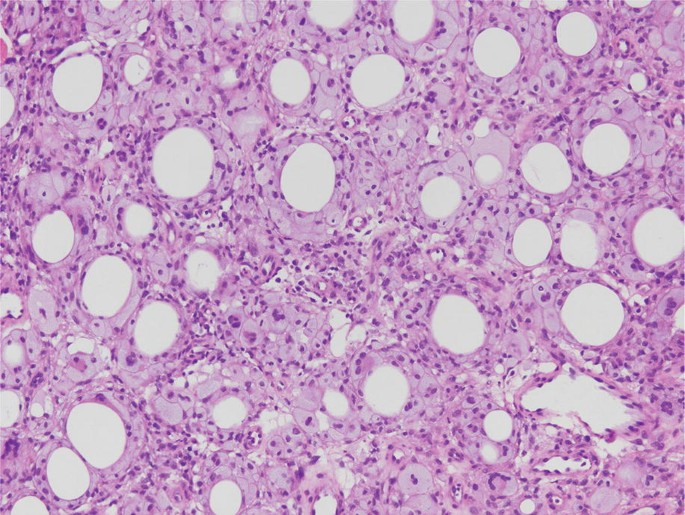
\includegraphics[width=\textwidth]{../Task1.jpg}
    \captionof{figure}{Original image}
    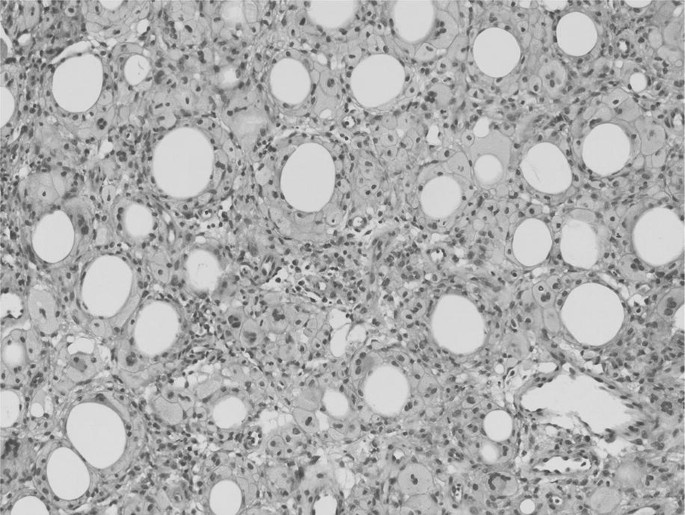
\includegraphics[width=\textwidth]{../code/task1/output/greyscale.jpg}
    \captionof{figure}{Greyscale original}
\end{minipage}
\hfill
\begin{minipage}{0.24\textwidth}
    \centering
    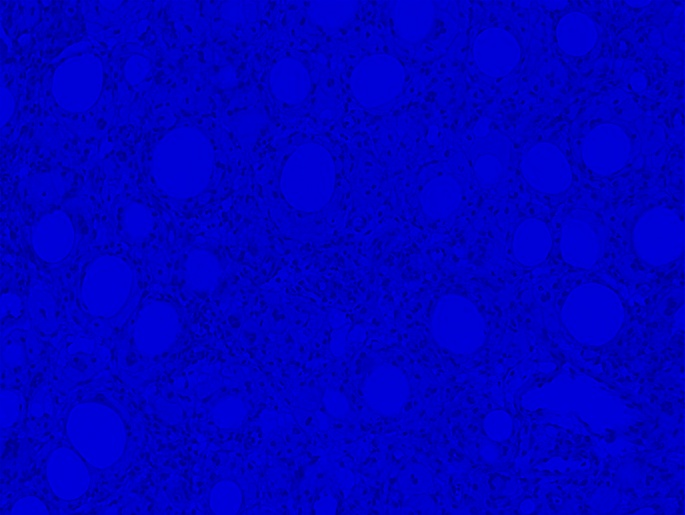
\includegraphics[width=\textwidth]{../code/task1/output/b_channel.jpg}
    \captionof{figure}{B-Channel}
    
\includegraphics[width=\textwidth]{../code/task1/output/b_channel_greyscale.jpg}
    \captionof{figure}{B-Greyscale}
\end{minipage}
\hfill
\begin{minipage}{0.24\textwidth}
    \centering
    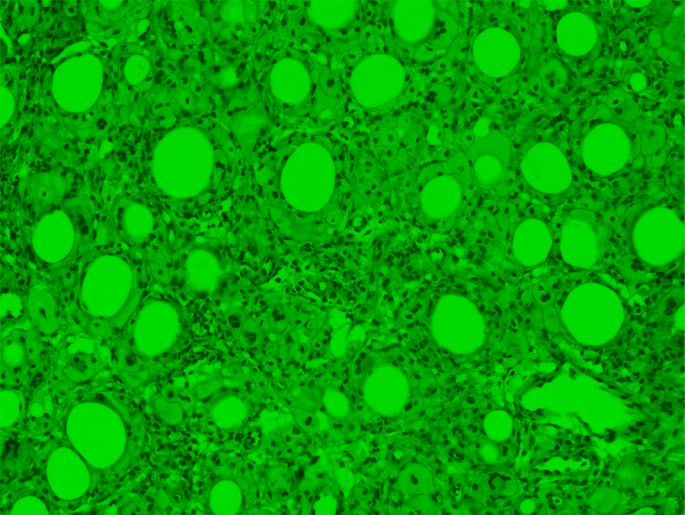
\includegraphics[width=\textwidth]{../code/task1/output/g_channel.jpg}
    \captionof{figure}{G-Channel}
    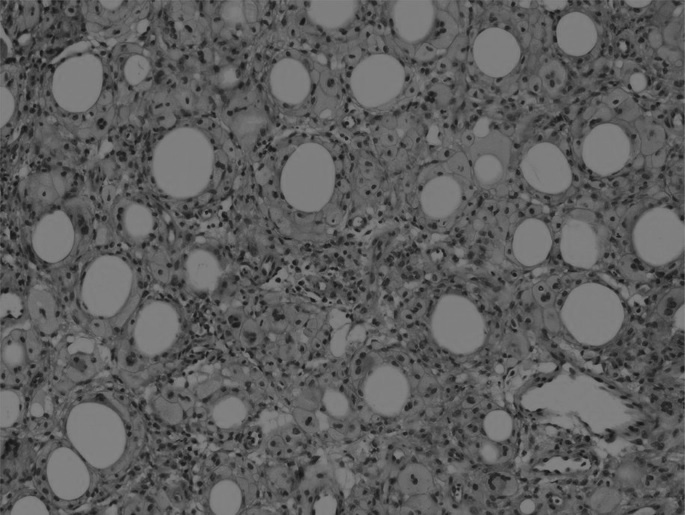
\includegraphics[width=\textwidth]{../code/task1/output/g_channel_greyscale.jpg}
    \captionof{figure}{G-Greyscale}
\end{minipage}
\hfill
\begin{minipage}{0.24\textwidth}
    \centering
    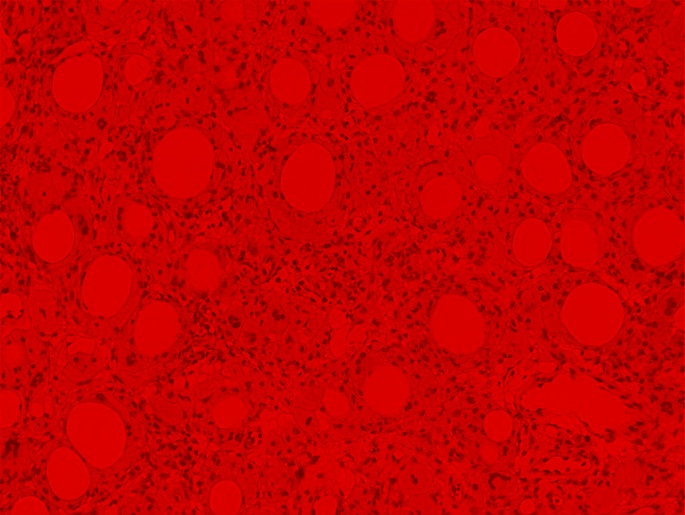
\includegraphics[width=\textwidth]{../code/task1/output/r_channel.jpg}
    \captionof{figure}{R-Channel}
    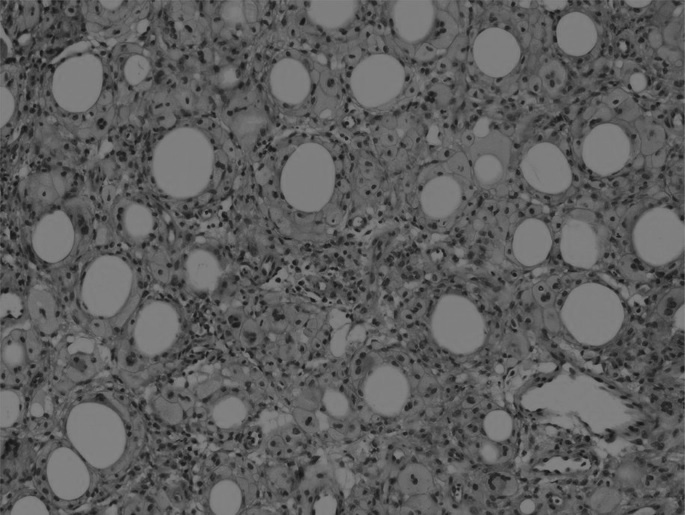
\includegraphics[width=\textwidth]{../code/task1/output/r_channel_greyscale.jpg}
    \captionof{figure}{R-Greyscale}
\end{minipage}

My selected single-channel image is the greyscale version of the green-channel-only image, as it yields the greatest contrast:
\begin{figure}[H]
    \centering
    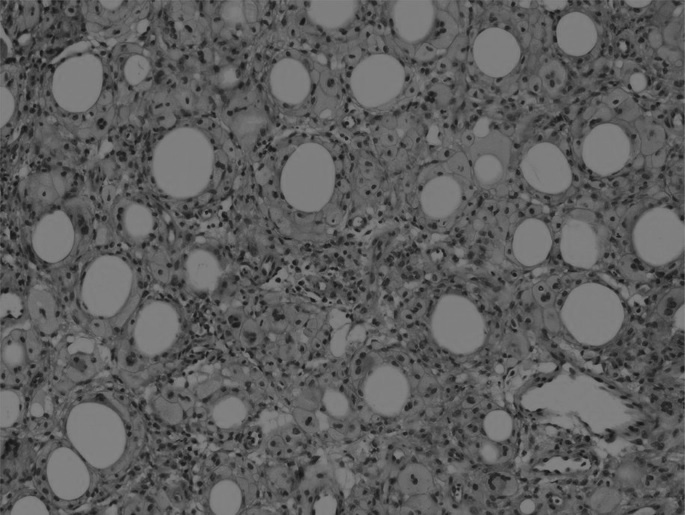
\includegraphics[width=0.5\textwidth]{../code/task1/output/g_channel_greyscale.jpg}
    \caption{Selected single-channel image: greyscale green-channel-only}
\end{figure}

\subsection{Image Enhancement}

\end{document}
